%%
%% VIDAR: Vulnerability Identification, Developer Assessment, and Risk
%%        Quantification Framework for Vibe-Coded Software Platforms
%%
%% Target: Journal of Systems and Software (Elsevier)
%%         Special Issue: "Reliable and Secure LLMs for SE"
%%         Submission type: VSI:Reliable and Secure LLMs for SE
%%
%% Template: elsarticle (Elsevier)
%%

\documentclass[preprint,review,12pt]{elsarticle}

%% Packages
\usepackage{amssymb}
\usepackage{amsmath}
\usepackage{graphicx}
\usepackage{booktabs}
\usepackage{multirow}
\usepackage{array}
\usepackage{tabularx}
\usepackage{xcolor}
\usepackage{hyperref}
\usepackage{tikz}
\usetikzlibrary{shapes.geometric, arrows.meta, positioning, fit, backgrounds, calc}
\usepackage{pgfplots}
\pgfplotsset{compat=1.18}
\usepgfplotslibrary{polar}
\usepackage{enumitem}
\usepackage{subcaption}
\usepackage{rotating}
\usepackage{longtable}
%\usepackage{lineno}

%% Line numbers for review (disabled)
%\modulolinenumbers[5]

%% Journal name
\journal{Journal of Systems and Software}

%% Natbib for numerical citations
\bibliographystyle{elsarticle-num}

%% Custom commands
\newcommand{\vidar}{\textsc{Vidar}}
\newcommand{\vrs}{\textit{VRS}}
\newcommand{\dcd}{\textit{DCD}}
\newcommand{\abi}{\textit{ABI}}
\newcommand{\sir}{\textit{SIR}}
\newcommand{\idr}{\textit{IDR}}
\newcommand{\hri}{\textit{HRI}}

\begin{document}

\begin{frontmatter}

%% Title
\title{VIDAR: A Multi-Dimensional Risk Assessment Framework for Vibe-Coded Software Platforms with Bayesian Quantification and Developer Comprehension Modeling}

%% Authors
\author[uok]{Hiruni Hathnagoda\corref{cor1}}
\ead{hirunih99@gmail.com}

\author[uok]{Ruwan Wickramarachchi}
\ead{ruwan@kln.ac.lk}

\cortext[cor1]{Corresponding author}

\affiliation[uok]{organization={Department of Industrial Management, Faculty of Science, University of Kelaniya},
            city={Kelaniya},
            country={Sri Lanka}}

%% Abstract
\begin{abstract}
The rapid adoption of ``vibe coding'' --- generating software through natural language prompts to large language models (LLMs) --- has democratized software development while introducing unprecedented security risks. Empirical studies report that 40--62\% of AI-generated code contains security vulnerabilities, with only 10.5\% of functionally correct vibe-coded solutions meeting security requirements. Despite these alarming findings, no comprehensive, quantitative risk assessment framework exists specifically for vibe-coded platforms. This paper presents \vidar{} (\textbf{V}ulnerability \textbf{I}dentification, \textbf{D}eveloper \textbf{A}ssessment, and \textbf{R}isk quantification), a multi-dimensional framework for systematic risk assessment of vibe-coded software platforms. Building on our prior work classifying security risks in low-code development platforms (LCDPs) across four categories, \vidar{} extends and transforms this taxonomy into six risk dimensions encompassing 28+ measurable risk factors: Code Generation Security, Data \& Model Security, Platform \& Toolchain, Developer \& Human Factors, Generative Process, and Governance \& Organizational. At its core, a three-tier Bayesian network engine, augmented with fuzzy membership functions and Analytic Hierarchy Process weighting, produces a quantitative \vidar{} Risk Score (VRS) in $[0, 1]$ for any given platform--project--developer configuration. The framework introduces novel metrics including the Developer Comprehension Deficit (DCD) and Automation Bias Index (ABI) to formally quantify human-factor risks unique to AI-assisted development. We validate \vidar{} through a six-phase mixed-methods methodology: systematic literature review, expert Delphi study, empirical platform benchmarking across six vibe coding platforms using static and dynamic analysis tools, Bayesian network calibration and sensitivity analysis, case study application, and practitioner evaluation. Results demonstrate that \vidar{} provides differentiated, actionable risk profiles across platforms and that developers with lower comprehension scores produce significantly riskier deployments. This work contributes the first comprehensive, empirically validated, quantitative risk assessment framework bridging the ``democratized development risk continuum'' from low-code to vibe-code paradigms.
\end{abstract}

%%Graphical abstract (optional)
%\begin{graphicalabstract}
%\end{graphicalabstract}

%% Keywords
\begin{keyword}
vibe coding \sep AI-generated code security \sep risk assessment framework \sep Bayesian network \sep developer comprehension \sep low-code development platforms
\end{keyword}

\end{frontmatter}

%% Line numbering (disabled)
%\linenumbers

%% ============================================================================
%% SECTION 1: INTRODUCTION
%% ============================================================================
\section{Introduction}
\label{sec:introduction}

Software development is undergoing its most significant paradigm shift since the introduction of high-level programming languages. The emergence of ``vibe coding'' --- a term coined by Andrej Karpathy in February 2025 \cite{karpathy2025vibe} to describe the practice of generating software through natural language conversations with large language models (LLMs) --- has fundamentally altered who can create software and how it is produced. Platforms such as GitHub Copilot, Cursor, Claude Code, Replit, Windsurf, and Lovable now enable developers and non-developers alike to produce functional applications by describing desired behavior in plain English, with the AI handling the translation to executable code.

The scale and velocity of this transformation are remarkable. Industry analyses indicate that AI-assisted code generation is being adopted across organizations of all sizes, with Gartner predicting that by 2028, AI-generated code will account for a substantial portion of all new software, leading to a projected 2500\% increase in software defects \cite{gartner2026defects}. This explosive growth is driven by the same forces that propelled low-code development platforms (LCDPs) to a projected \$26 billion market \cite{gartner2024lowcode}: the democratization of software creation for users with limited traditional programming expertise.

However, this democratization carries severe security implications. Empirical research has consistently demonstrated that AI-generated code harbors significant vulnerabilities. Pearce et al.\ \cite{pearce2022asleep} found that approximately 40\% of GitHub Copilot's code suggestions contained security weaknesses. Perry et al.\ \cite{perry2023users} showed that developers using AI assistants produced significantly less secure code while paradoxically expressing greater confidence in their output. Most alarmingly, Jiang et al.\ \cite{jiang2025vibecoding} conducted the largest empirical study of vibe-coded programs to date, finding that only 10.5\% of functionally correct solutions met security requirements --- revealing a fundamental tension between functional correctness and security in the vibe coding paradigm.

Despite these findings, the current landscape of security frameworks and risk assessment tools fails to adequately address the unique risks of vibe-coded software. Existing frameworks such as the OWASP Top 10 for LLM Applications \cite{owasp2025llm} focus on LLM deployment risks rather than code generation security. The SHIELD framework \cite{unit42shield} provides qualitative guidance but lacks quantitative risk scoring. The NIST AI Risk Management Framework \cite{nist2023ai} offers broad AI governance principles without vibe-coding-specific operationalization. No existing framework simultaneously addresses all critical dimensions: the security of generated code, the risks of the generative process itself, platform-specific variations, developer comprehension gaps, and organizational governance challenges.

This gap is especially concerning given the trajectory we identified in our prior work. In Hathnagoda and Wickramarachchi \cite{hathnagoda2024assessing}, we conducted a systematic literature review of security risks in seven leading LCDPs (Mendix, OutSystems, Microsoft Power Apps, ServiceNow, Salesforce, Oracle, and Pegasystems), classifying risks into four categories: Application Security Risks, Information Security Risks, Platform-Specific Risks, and User-Related Risks. That work revealed how the democratization of development through LCDPs inherently creates security vulnerabilities when non-professional developers lack the expertise to implement secure coding practices. Vibe coding amplifies every risk dimension we identified while introducing entirely new categories of risk --- particularly around AI hallucination, prompt engineering failures, and the erosion of developer code comprehension.

This paper presents \vidar{} (\textbf{V}ulnerability \textbf{I}dentification, \textbf{D}eveloper \textbf{A}ssessment, and \textbf{R}isk quantification), a comprehensive, multi-dimensional risk assessment framework designed specifically for vibe-coded software platforms. \vidar{} makes three primary contributions:

\begin{enumerate}[label=\textbf{C\arabic*.}]
    \item \textbf{A six-dimension risk taxonomy} with 28+ formally defined, measurable risk factors that extends and transforms the LCDP risk categories into the vibe coding context, adding two entirely new dimensions (Generative Process and Governance \& Organizational) that have no direct LCDP analogue.

    \item \textbf{A Bayesian-fuzzy hybrid quantification engine} that produces a quantitative \vidar{} Risk Score (VRS) in $[0,1]$, enabling objective comparison across platforms, projects, and organizational contexts --- the first such quantitative scoring mechanism for vibe-coded software.

    \item \textbf{Novel human-factor risk metrics} --- the Developer Comprehension Deficit (DCD) and Automation Bias Index (ABI) --- that formally quantify the unique cognitive and behavioral risks introduced when developers deploy code they may not fully understand.
\end{enumerate}

The remainder of this paper is organized as follows. Section~\ref{sec:background} establishes the background and positions \vidar{} against related work. Section~\ref{sec:methodology} details our six-phase mixed-methods research methodology. Section~\ref{sec:framework} presents the \vidar{} framework in full. Section~\ref{sec:validation} reports validation results. Section~\ref{sec:discussion} discusses implications and limitations. Section~\ref{sec:conclusion} concludes with contributions and future directions.

%% ============================================================================
%% SECTION 2: BACKGROUND AND RELATED WORK
%% ============================================================================
\section{Background and Related Work}
\label{sec:background}

\subsection{The Democratized Development Risk Continuum}
\label{subsec:continuum}

Software development has progressed through distinct paradigms of increasing accessibility, each expanding the pool of potential developers while simultaneously introducing new categories of security risk. We conceptualize this progression as the \textit{Democratized Development Risk Continuum} (Fig.~\ref{fig:continuum}), a theoretical framework connecting three major paradigms:

\textbf{Traditional Development} relies on professional developers writing code manually in general-purpose programming languages. Security risks are well-understood and addressed by mature frameworks (OWASP, SANS, CWE), but the high barrier to entry limits who can create software.

\textbf{Low-Code/No-Code Development} emerged to bridge this gap, providing visual development environments with pre-built components that enable ``citizen developers'' to create applications with minimal coding \cite{woo2020rise, sahay2020supporting}. As our prior work demonstrated \cite{hathnagoda2024assessing}, this democratization introduced four categories of security risk --- application, information, platform-specific, and user-related --- driven primarily by the gap between the platform's ease of use and the security expertise required to deploy applications safely.

\textbf{Vibe Coding} represents the latest and most radical step in this continuum. By replacing visual builders with natural language prompts, vibe coding further lowers the barrier while fundamentally changing the developer's relationship with the generated code. Unlike LCDP development, where users assemble visible components and can inspect the resulting application structure, vibe coding produces opaque code that developers may accept without full comprehension.

Critically, these paradigms are converging. Major LCDP vendors are integrating AI code generation capabilities: Microsoft Power Apps now incorporates Copilot, Salesforce has introduced Einstein AI, and Mendix has added AI-assisted development features. This convergence creates hybrid platforms that inherit risks from both the LCDP and vibe coding paradigms, making a unified risk framework essential.

\begin{figure}[t]
\centering
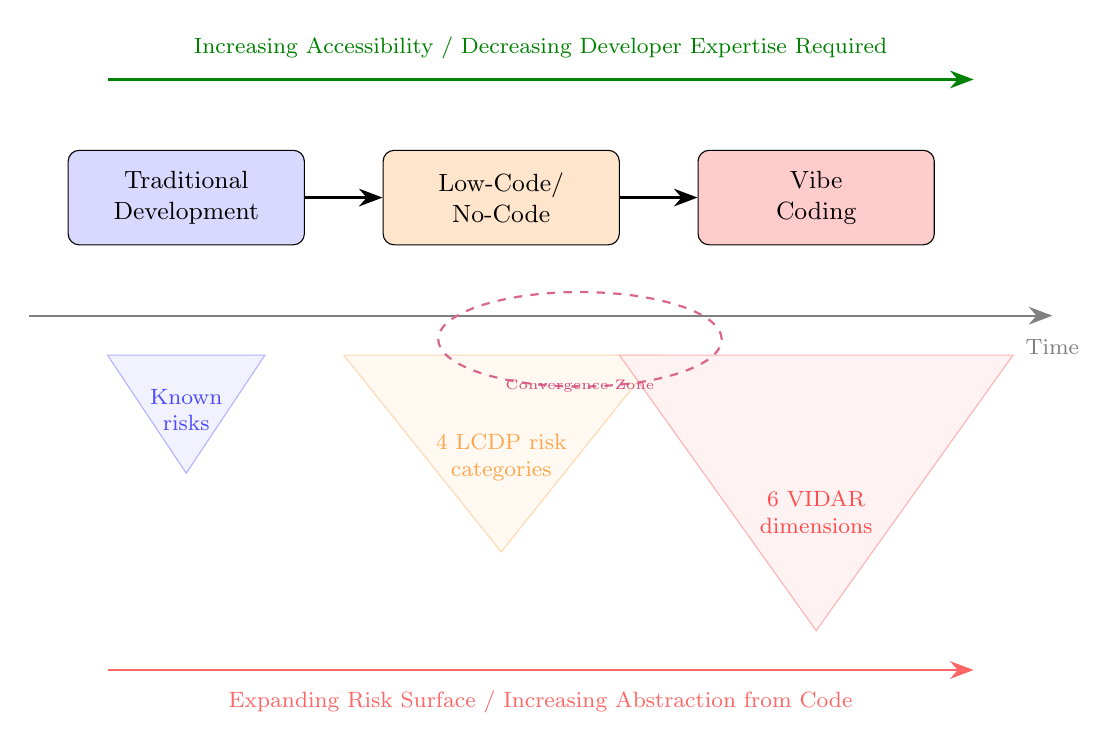
\begin{tikzpicture}[
    node distance=2.5cm,
    >={Stealth[length=3mm]},
    box/.style={rectangle, rounded corners, draw=black, fill=#1, minimum width=3cm, minimum height=1.2cm, align=center, font=\small},
    label/.style={font=\footnotesize, align=center, text width=3.5cm}
]
% Timeline arrow
\draw[->, thick, gray] (-0.5, 0) -- (12.5, 0);
\node[font=\footnotesize, gray] at (12.5, -0.4) {Time};

% Paradigm boxes
\node[box=blue!15] (trad) at (1.5, 1.5) {Traditional\\Development};
\node[box=orange!20] (lcdp) at (5.5, 1.5) {Low-Code/\\No-Code};
\node[box=red!20] (vibe) at (9.5, 1.5) {Vibe\\Coding};

% Risk expansion cones (simplified as triangles)
\draw[blue!30, fill=blue!5] (0.5, -0.5) -- (2.5, -0.5) -- (1.5, -2.0) -- cycle;
\draw[orange!30, fill=orange!5] (3.5, -0.5) -- (7.5, -0.5) -- (5.5, -3.0) -- cycle;
\draw[red!30, fill=red!5] (7.0, -0.5) -- (12.0, -0.5) -- (9.5, -4.0) -- cycle;

% Risk labels
\node[label, blue!70] at (1.5, -1.2) {Known\\risks};
\node[label, orange!70] at (5.5, -1.8) {4 LCDP risk\\categories};
\node[label, red!70] at (9.5, -2.5) {6 VIDAR\\dimensions};

% Convergence zone
\draw[dashed, thick, purple!60] (6.5, -0.3) ellipse (1.8cm and 0.6cm);
\node[font=\tiny, purple!70, text width=3cm, align=center] at (6.5, -0.9) {Convergence Zone};

% Arrows between paradigms
\draw[->, thick] (trad) -- (lcdp);
\draw[->, thick] (lcdp) -- (vibe);

% Accessibility label
\draw[->, thick, green!50!black] (0.5, 3) -- (11.5, 3);
\node[font=\footnotesize, green!50!black] at (6, 3.4) {Increasing Accessibility / Decreasing Developer Expertise Required};

% Risk label
\draw[->, thick, red!60] (0.5, -4.5) -- (11.5, -4.5);
\node[font=\footnotesize, red!60] at (6, -4.9) {Expanding Risk Surface / Increasing Abstraction from Code};

\end{tikzpicture}
\caption{The Democratized Development Risk Continuum: as software development paradigms evolve toward greater accessibility, the risk surface expands. The convergence zone indicates where LCDP vendors integrate AI code generation, creating hybrid risk profiles.}
\label{fig:continuum}
\end{figure}


\subsection{The Vibe Coding Ecosystem}
\label{subsec:vibecoding}

Vibe coding, as defined by Karpathy \cite{karpathy2025vibe}, refers to a development paradigm where the programmer ``fully gives in to the vibes, embraces exponentials, and forgets that the code even exists.'' In practice, this manifests as developers using LLM-powered tools to generate, modify, and debug code through conversational natural language interfaces, often accepting the AI's output with minimal manual review.

The current vibe coding ecosystem comprises several platform categories:

\begin{itemize}
    \item \textbf{IDE-integrated assistants:} GitHub Copilot, Cursor, Windsurf (Codeium), and Claude Code, which augment traditional development environments with AI code generation and chat-based assistance.
    \item \textbf{Standalone generation platforms:} Replit, Lovable (formerly GPT Engineer), Bolt, and v0 by Vercel, which enable end-to-end application creation from natural language specifications.
    \item \textbf{AI-enhanced LCDPs:} Microsoft Power Apps with Copilot, Salesforce with Einstein AI, and Mendix with AI-assisted development, representing the convergence of LCDP and vibe coding paradigms.
    \item \textbf{General-purpose LLMs used for coding:} ChatGPT, Claude, and Gemini used directly for code generation through conversational interfaces.
\end{itemize}

Each category presents distinct risk profiles based on the level of abstraction, the degree of developer control, the transparency of generated code, and the integration with security tooling.

\subsection{Security of AI-Generated Code}
\label{subsec:aisecurity}

A growing body of empirical research has documented the security implications of AI-generated code. Table~\ref{tab:empirical_security} summarizes key findings.

\begin{table}[t]
\centering
\caption{Empirical findings on AI-generated code security.}
\label{tab:empirical_security}
\footnotesize
\begin{tabular}{p{3cm} p{4cm} p{4cm}}
\toprule
\textbf{Study} & \textbf{Scope} & \textbf{Key Finding} \\
\midrule
Pearce et al.\ \cite{pearce2022asleep} & Copilot, 89 CWE scenarios & $\sim$40\% of suggestions contained vulnerabilities \\
Perry et al.\ \cite{perry2023users} & 47 participants, 5 tasks & AI users wrote significantly less secure code; higher confidence \\
Sandoval et al.\ \cite{sandoval2023lost} & 58 participants, C programming & No significant security difference, but AI users less likely to identify bugs \\
Jiang et al.\ \cite{jiang2025vibecoding} & Large-scale vibe coding study & Only 10.5\% of correct solutions were secure \\
Fu et al.\ \cite{fu2023security} & Copilot in GitHub projects & Prevalent CWEs: injection, XSS, path traversal \\
Tony et al.\ \cite{tony2023llmseceval} & LLMSecEval benchmark & 62\% of generated code contained at least one CWE \\
\bottomrule
\end{tabular}
\end{table}

These studies reveal several consistent patterns: (1) AI-generated code frequently contains vulnerabilities from established CWE categories; (2) developers using AI assistants tend to exhibit automation bias, trusting AI output more than warranted; (3) the iterative, conversational nature of vibe coding can compound security issues across interaction turns; and (4) non-deterministic generation means the same prompt can produce code with varying security properties.

\subsection{Existing Security Frameworks and Standards}
\label{subsec:frameworks}

Several frameworks address aspects of AI and software security, but none comprehensively covers the vibe coding risk landscape.

The \textbf{OWASP Top 10 for LLM Applications} \cite{owasp2025llm} identifies risks such as prompt injection, insecure output handling, and training data poisoning. While relevant, it focuses on LLM \textit{deployment} risks rather than the security of code \textit{generated by} LLMs.

The \textbf{SHIELD framework} \cite{unit42shield} from Palo Alto Networks' Unit 42 directly addresses AI-generated code security with practical guidance for securing vibe-coded applications. However, it provides qualitative recommendations without quantitative scoring or platform-specific differentiation.

The \textbf{NIST AI Risk Management Framework} \cite{nist2023ai} and its \textbf{Generative AI Profile} \cite{nist2024genai} offer comprehensive governance principles for AI systems but require significant operationalization to apply specifically to vibe coding scenarios.

The \textbf{Cloud Security Alliance (CSA) Guide} \cite{csa2024ai} provides best practices for securing AI-generated code but lacks a structured risk quantification methodology.

The \textbf{FAIR model} \cite{freund2014measuring} and its Bayesian network extensions \cite{fair2024bn} provide rigorous quantitative risk analysis methodology, which we adapt for the vibe coding context.

The \textbf{SusVibes framework} \cite{alomar2025susvibes} addresses sustainability aspects of vibe-coded software, including partial security considerations, but is not designed as a comprehensive security risk assessment tool.

\subsection{Gap Analysis}
\label{subsec:gap}

Table~\ref{tab:framework_comparison} presents a systematic comparison of existing frameworks against the requirements for comprehensive vibe coding risk assessment. The analysis reveals that no existing framework simultaneously provides: (1) vibe-coding-specific risk identification, (2) quantitative risk scoring, (3) platform-aware differentiation, (4) developer comprehension modeling, (5) governance considerations, and (6) empirical validation. \vidar{} is designed to address all six requirements.

\begin{table}[t]
\centering
\caption{Comparison of existing frameworks against vibe coding risk assessment requirements. \checkmark\ = fully addressed; $\sim$ = partially addressed; --- = not addressed.}
\label{tab:framework_comparison}
\footnotesize
\begin{tabular}{p{3.2cm} c c c c c c c c}
\toprule
\textbf{Property} & \rotatebox{70}{\textbf{OWASP LLM}} & \rotatebox{70}{\textbf{SHIELD}} & \rotatebox{70}{\textbf{CSA Guide}} & \rotatebox{70}{\textbf{GRASP}} & \rotatebox{70}{\textbf{NIST AI RMF}} & \rotatebox{70}{\textbf{SusVibes}} & \rotatebox{70}{\textbf{VIDAR}} \\
\midrule
Vibe-coding specific     & $\sim$ & \checkmark & \checkmark & --- & --- & \checkmark & \checkmark \\
Quantitative scoring      & --- & --- & --- & --- & --- & $\sim$ & \checkmark \\
Platform-aware profiles   & --- & --- & --- & --- & --- & $\sim$ & \checkmark \\
Developer comprehension   & --- & $\sim$ & --- & --- & --- & --- & \checkmark \\
Governance dimension      & --- & $\sim$ & $\sim$ & --- & \checkmark & --- & \checkmark \\
Connected to LCDP lit.    & --- & --- & --- & --- & --- & --- & \checkmark \\
Bayesian dependency model & --- & --- & --- & --- & --- & --- & \checkmark \\
Empirically validated     & N/A & --- & --- & \checkmark & N/A & \checkmark & \checkmark \\
\bottomrule
\end{tabular}
\end{table}


%% ============================================================================
%% SECTION 3: RESEARCH METHODOLOGY
%% ============================================================================
\section{Research Methodology}
\label{sec:methodology}

This study employs a six-phase mixed-methods research design \cite{creswell2017research} that combines systematic literature review, expert consultation, empirical benchmarking, probabilistic modeling, case study application, and practitioner evaluation. Fig.~\ref{fig:methodology} illustrates the overall research design and the relationships between phases.

\begin{figure}[t]
\centering
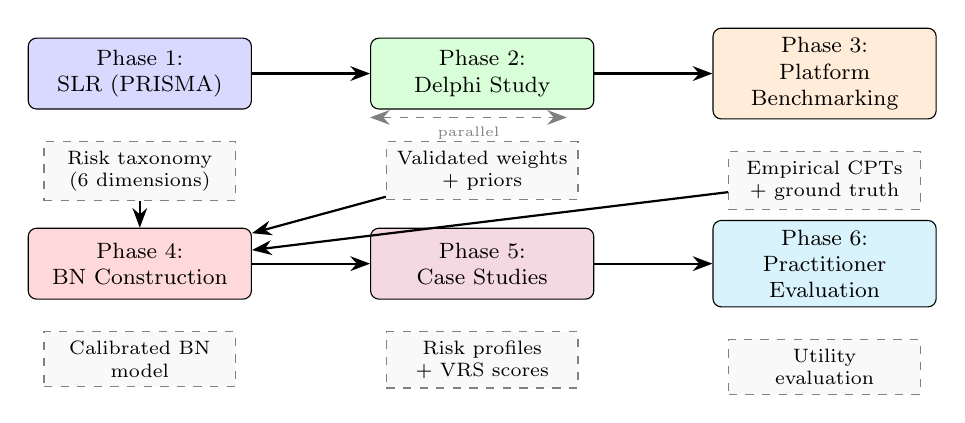
\begin{tikzpicture}[
    node distance=1.0cm and 1.5cm,
    >={Stealth[length=2.5mm]},
    phase/.style={rectangle, rounded corners=3pt, draw=black, fill=#1, minimum width=2.8cm, minimum height=0.9cm, align=center, font=\footnotesize, text width=2.6cm},
    output/.style={rectangle, draw=gray, dashed, fill=gray!5, minimum width=2.4cm, minimum height=0.7cm, align=center, font=\scriptsize, text width=2.2cm},
    arrow/.style={->, thick}
]

% Phase boxes
\node[phase=blue!15] (p1) {Phase 1:\\SLR (PRISMA)};
\node[phase=green!15, right=of p1] (p2) {Phase 2:\\Delphi Study};
\node[phase=orange!15, right=of p2] (p3) {Phase 3:\\Platform\\Benchmarking};
\node[phase=red!15, below=1.5cm of p1] (p4) {Phase 4:\\BN Construction};
\node[phase=purple!15, right=of p4] (p5) {Phase 5:\\Case Studies};
\node[phase=cyan!15, right=of p5] (p6) {Phase 6:\\Practitioner\\Evaluation};

% Outputs
\node[output, below=0.4cm of p1] (o1) {Risk taxonomy\\(6 dimensions)};
\node[output, below=0.4cm of p2] (o2) {Validated weights\\+ priors};
\node[output, below=0.4cm of p3] (o3) {Empirical CPTs\\+ ground truth};
\node[output, below=0.4cm of p4] (o4) {Calibrated BN\\model};
\node[output, below=0.4cm of p5] (o5) {Risk profiles\\+ VRS scores};
\node[output, below=0.4cm of p6] (o6) {Utility\\evaluation};

% Arrows
\draw[arrow] (p1) -- (p2);
\draw[arrow] (p2) -- (p3);
\draw[arrow] (o1) -- (p4);
\draw[arrow] (o2) -- (p4);
\draw[arrow] (o3) -- (p4);
\draw[arrow] (p4) -- (p5);
\draw[arrow] (p5) -- (p6);

% Parallel indicator
\draw[<->, dashed, gray] (p2.south west) ++(0,-0.1) -- ++(2.5,0) node[midway, below, font=\tiny, gray] {parallel};

\end{tikzpicture}
\caption{Six-phase mixed-methods research design. Phases 2 and 3 execute in parallel; their outputs converge to inform Bayesian network construction in Phase 4.}
\label{fig:methodology}
\end{figure}


\subsection{Phase 1: Systematic Literature Review}
\label{subsec:phase1}

We conduct a systematic literature review following the PRISMA 2020 guidelines \cite{page2021prisma} to establish the evidence base for the \vidar{} risk taxonomy.

\textbf{Search strategy.} We search five academic databases --- IEEE Xplore, ACM Digital Library, ScienceDirect, Springer Link, and arXiv --- using the query:

\begin{quote}
\small
\texttt{("vibe coding" OR "AI-generated code" OR "LLM code generation" OR "AI-assisted development" OR "copilot security" OR "AI coding assistant") AND ("security" OR "vulnerability" OR "risk" OR "safety")}
\end{quote}

The search scope covers publications from January 2022 to December 2026, reflecting the recency of the vibe coding phenomenon.

\textbf{Inclusion criteria:} (IC1) Publications addressing security aspects of AI-generated or AI-assisted code; (IC2) Peer-reviewed journal articles, conference papers, and high-quality preprints (arXiv with $\geq$10 citations); (IC3) Publications in English; (IC4) Studies covering at least one vibe coding platform or LLM code generation tool.

\textbf{Exclusion criteria:} (EC1) Studies focusing exclusively on LLM deployment security without code generation aspects; (EC2) Non-peer-reviewed opinion pieces or blog posts; (EC3) Studies predating practical LLM code generation tools (pre-2022); (EC4) Duplicate or substantially overlapping publications.

\textbf{Data extraction} maps each identified risk to one or more of the six \vidar{} dimensions, recording: risk factor name, description, affected dimension(s), evidence type (empirical/theoretical), severity indicators, and platform specificity.


\subsection{Phase 2: Expert Validation (Modified Delphi Study)}
\label{subsec:phase2}

We employ a modified Delphi method \cite{linstone1975delphi, diamond2014defining} with 15--20 experts drawn from three communities: AI security researchers, software engineering practitioners with vibe coding experience, and risk management professionals.

The Delphi study serves three purposes:
\begin{enumerate}
    \item \textbf{Taxonomy validation:} Experts evaluate the completeness and correctness of the six-dimension risk taxonomy, suggesting additions, removals, or reclassifications.
    \item \textbf{AHP weight elicitation:} Using the Analytic Hierarchy Process \cite{saaty1980ahp, saaty2008ahp}, experts perform pairwise comparisons of the six dimensions to derive importance weights $w_i$ for the VRS formula.
    \item \textbf{Prior probability estimation:} Experts provide initial probability estimates for risk factor nodes in the Bayesian network, establishing prior distributions where empirical data is unavailable.
\end{enumerate}

Three Delphi rounds are conducted: Round 1 (open-ended risk identification and initial ratings), Round 2 (structured feedback with anonymized group statistics), and Round 3 (final convergence on weights and probabilities). Consensus is defined as $\geq$75\% agreement with interquartile range $\leq 1$ on a 5-point Likert scale.


\subsection{Phase 3: Empirical Platform Benchmarking}
\label{subsec:phase3}

We conduct controlled empirical benchmarking across six primary vibe coding platforms and two LCDP--AI hybrid platforms:

\textbf{Primary platforms:} (1) GitHub Copilot, (2) Cursor, (3) Claude Code, (4) Replit, (5) Windsurf, (6) Lovable.

\textbf{Hybrid LCDP--AI platforms:} (7) Microsoft Power Apps with Copilot, (8) Salesforce with Einstein AI.

\textbf{Benchmark applications.} We design a standardized suite of application specifications spanning common vulnerability categories:
\begin{itemize}
    \item A web application with user authentication and session management (targeting CWE-287, CWE-384)
    \item A data processing API with input handling (targeting CWE-89, CWE-79, CWE-78)
    \item A file management system with access controls (targeting CWE-22, CWE-732)
    \item A payment processing module with sensitive data handling (targeting CWE-311, CWE-312)
\end{itemize}

Each specification is submitted to each platform using identical natural language prompts, and the generated code is analyzed using:
\begin{itemize}
    \item \textbf{SAST:} Semgrep \cite{semgrep2024} and CodeQL \cite{codeql2024} for static vulnerability detection
    \item \textbf{DAST:} OWASP ZAP \cite{owaspzap2024} for dynamic runtime vulnerability scanning
    \item \textbf{Dependency auditing:} npm audit, pip-audit, and Snyk for supply chain risk assessment
    \item \textbf{Manual code review:} Two independent security reviewers assess each generated codebase
\end{itemize}

The benchmarking produces empirical conditional probability table (CPT) values for the Bayesian network leaf nodes, grounded in observed vulnerability rates.


\subsection{Phase 4: Bayesian Network Construction and Validation}
\label{subsec:phase4}

We construct the three-tier Bayesian network using PyAgrum \cite{brouillard2020pyagrum} and GeNIe \cite{genie2024}. The construction process involves:

\begin{enumerate}
    \item \textbf{Structure learning:} The DAG structure is specified based on the six-dimension taxonomy (expert-informed), with cross-dimension dependencies identified through expert elicitation and correlation analysis of empirical data.
    \item \textbf{Parameter learning:} CPTs are populated using a hybrid approach combining empirical frequencies from Phase 3 benchmarking with expert-elicited priors from Phase 2, using Bayesian updating.
    \item \textbf{Validation:} The model is validated through (a) sensitivity analysis via entropy reduction \cite{marcot2012metrics, marcot2019advances} to identify the most influential risk factors, (b) cross-validation against held-out empirical data, and (c) face validation by domain experts.
\end{enumerate}


\subsection{Phase 5: Case Study Application}
\label{subsec:phase5}

\vidar{} is applied to 2--3 real-world vibe-coded projects of varying complexity and domain. For each case study, we:
\begin{enumerate}
    \item Characterize the project context (platform, developer profile, organizational maturity)
    \item Instantiate the Bayesian network with project-specific evidence
    \item Compute the VRS and dimension-level risk scores
    \item Generate a risk profile radar chart and prioritized mitigation plan
    \item Compare the computed risk assessment against actual vulnerabilities discovered through independent security audit
\end{enumerate}


\subsection{Phase 6: Practitioner Evaluation}
\label{subsec:phase6}

We evaluate \vidar{}'s practical utility through a survey and semi-structured interviews with 20--30 software engineering and security practitioners. The evaluation employs the Technology Acceptance Model (TAM) \cite{davis1989tam} to assess perceived usefulness, perceived ease of use, and intention to adopt. Qualitative interview data is analyzed using thematic analysis to identify strengths, limitations, and improvement opportunities.


%% ============================================================================
%% SECTION 4: THE VIDAR FRAMEWORK
%% ============================================================================
\section{The VIDAR Framework}
\label{sec:framework}

\subsection{Overview and Design Principles}
\label{subsec:overview}

\vidar{} (\textbf{V}ulnerability \textbf{I}dentification, \textbf{D}eveloper \textbf{A}ssessment, and \textbf{R}isk quantification) is a multi-dimensional risk assessment framework structured as a four-layer process operating across six risk dimensions (Fig.~\ref{fig:architecture}). The framework is governed by five design principles:

\begin{enumerate}[label=\textbf{DP\arabic*.}]
    \item \textbf{Comprehensiveness:} Cover all significant risk sources, including those unique to the generative AI paradigm.
    \item \textbf{Quantifiability:} Produce measurable, comparable risk scores rather than qualitative labels alone.
    \item \textbf{Platform-awareness:} Accommodate the significant variation in risk profiles across different vibe coding platforms.
    \item \textbf{Human-centricity:} Explicitly model the developer's role, comprehension level, and cognitive biases as first-class risk factors.
    \item \textbf{Actionability:} Map identified risks to concrete, prioritized mitigation strategies aligned with established standards.
\end{enumerate}


\subsubsection{Four Vertical Layers}

The four vertical layers correspond to the stages of the risk management process, aligned with ISO~31000 \cite{iso31000} and ISO/IEC~27005 \cite{iso27005}:

\begin{itemize}
    \item \textbf{Layer 1 --- Risk Identification:} Systematic enumeration of risks across all six dimensions, producing a structured risk register.
    \item \textbf{Layer 2 --- Risk Analysis:} Probabilistic and impact analysis of identified risks using the Bayesian network engine, producing conditional probability distributions.
    \item \textbf{Layer 3 --- Risk Evaluation:} Composite scoring via the fuzzy-Bayesian hybrid model, producing the VRS and dimension-level scores.
    \item \textbf{Layer 4 --- Risk Treatment:} Mitigation mapping and prioritization, producing actionable remediation plans aligned with NIST \cite{nist2023ai}, OWASP \cite{owasp2021top10}, and ISO standards.
\end{itemize}

\begin{figure}[t]
\centering
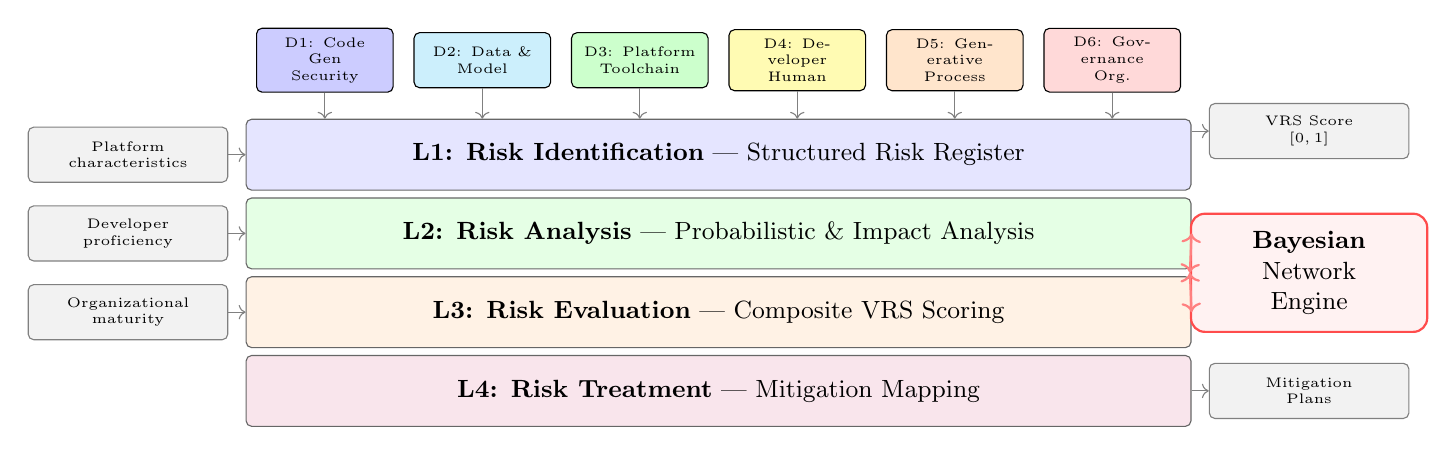
\begin{tikzpicture}[
    node distance=0.5cm,
    dim/.style={rectangle, rounded corners=2pt, draw=black, fill=#1, minimum width=1.6cm, minimum height=0.7cm, align=center, font=\tiny, text width=1.5cm},
    layer/.style={rectangle, rounded corners=2pt, draw=black!60, fill=#1, minimum width=12cm, minimum height=0.9cm, align=center, font=\small},
    engine/.style={rectangle, rounded corners=5pt, draw=red!70, fill=red!5, thick, minimum width=3cm, minimum height=1.5cm, align=center, font=\small},
    io/.style={rectangle, rounded corners=2pt, draw=gray, fill=gray!10, minimum width=2.5cm, minimum height=0.7cm, align=center, font=\tiny, text width=2.3cm}
]

% Layers
\node[layer=blue!10] (l1) at (0, 4) {\textbf{L1: Risk Identification} --- Structured Risk Register};
\node[layer=green!10] (l2) at (0, 3) {\textbf{L2: Risk Analysis} --- Probabilistic \& Impact Analysis};
\node[layer=orange!10] (l3) at (0, 2) {\textbf{L3: Risk Evaluation} --- Composite VRS Scoring};
\node[layer=purple!10] (l4) at (0, 1) {\textbf{L4: Risk Treatment} --- Mitigation Mapping};

% Dimensions across the top
\node[dim=blue!20] (d1) at (-5, 5.2) {D1: Code Gen\\Security};
\node[dim=cyan!20] (d2) at (-3, 5.2) {D2: Data \&\\Model};
\node[dim=green!20] (d3) at (-1, 5.2) {D3: Platform\\Toolchain};
\node[dim=yellow!30] (d4) at (1, 5.2) {D4: Developer\\Human};
\node[dim=orange!20] (d5) at (3, 5.2) {D5: Generative\\Process};
\node[dim=red!15] (d6) at (5, 5.2) {D6: Governance\\Org.};

% Dimension arrows down to L1
\foreach \d in {d1, d2, d3, d4, d5, d6}
    \draw[->, gray, thin] (\d.south) -- (\d.south |- l1.north);

% BN Engine
\node[engine] (bn) at (7.5, 2.5) {\textbf{Bayesian}\\Network\\Engine};
\draw[<->, thick, red!50] (l2.east) -- (bn.west);
\draw[<->, thick, red!50] (l3.east) -- (bn.west);

% Inputs
\node[io] (in1) at (-7.5, 4) {Platform\\characteristics};
\node[io] (in2) at (-7.5, 3) {Developer\\proficiency};
\node[io] (in3) at (-7.5, 2) {Organizational\\maturity};

\draw[->, gray] (in1.east) -- (l1.west |- in1.east);
\draw[->, gray] (in2.east) -- (l2.west |- in2.east);
\draw[->, gray] (in3.east) -- (l3.west |- in3.east);

% Outputs
\node[io] (out1) at (7.5, 4.3) {VRS Score\\$[0, 1]$};
\node[io] (out2) at (7.5, 1) {Mitigation\\Plans};

\draw[->, gray] (l1.east |- out1) -- (out1.west);
\draw[->, gray] (l4.east) -- (out2.west);

\end{tikzpicture}
\caption{VIDAR framework architecture: four vertical layers (risk management process) operate across six horizontal dimensions, with a Bayesian network engine at the core. Inputs (left) characterize the assessment context; outputs (right) include quantitative risk scores and actionable mitigation plans.}
\label{fig:architecture}
\end{figure}


\subsection{Six Risk Dimensions and Risk Factors}
\label{subsec:dimensions}

The six \vidar{} dimensions extend the four-category LCDP risk taxonomy from our prior work \cite{hathnagoda2024assessing} with two entirely new dimensions (D5, D6) that address risks unique to or significantly amplified by the vibe coding paradigm. Table~\ref{tab:dimensions} provides the complete taxonomy with evolutionary lineage.

\begin{table}[t]
\centering
\caption{VIDAR six-dimension risk taxonomy with LCDP lineage and representative risk factors.}
\label{tab:dimensions}
\footnotesize
\begin{tabular}{p{0.3cm} p{2.5cm} p{2.5cm} p{5.5cm}}
\toprule
\textbf{\#} & \textbf{Dimension} & \textbf{Evolves From} & \textbf{Key Risk Factors} \\
\midrule
D1 & Code Generation Security & Application Security Risks & Vulnerability Injection Rate; Semantic Infidelity Risk; Iterative Degradation Risk; Non-Deterministic Output Risk; XSS/Injection Generation Rate \\
\addlinespace
D2 & Data \& Model Security & Information Security Risks & Prompt Data Leakage; Training Data Contamination; Context Window Exploitation; Intellectual Property Exposure Risk \\
\addlinespace
D3 & Platform \& Toolchain & Platform-Specific Risks & Platform Security Posture Variance; Supply Chain Hallucination (Slopsquatting); Toolchain Integration Risk; Model Version Drift; Agentic Autonomy Risk \\
\addlinespace
D4 & Developer \& Human Factors & User-Related Risks & Developer Comprehension Deficit (DCD); Automation Bias Index (ABI); Security Skill Atrophy; Citizen Vibe-Coder Risk; Review Fatigue \\
\addlinespace
D5 & Generative Process & \textit{NEW --- no LCDP analogue} & Hallucination Risk Index; Prompt Engineering Risk; Context Loss/Fragmentation; Reproducibility/Auditability Risk; Model Capability Boundary Risk \\
\addlinespace
D6 & Governance \& Organizational & \textit{NEW --- extends beyond LCDP scope} & Policy Vacuum Risk; Accountability Gap; Regulatory Compliance (EU AI Act, NIST); Technical Debt Acceleration; Vendor Lock-In \\
\bottomrule
\end{tabular}
\end{table}


\subsubsection{D1: Code Generation Security}
\label{subsubsec:d1}

This dimension addresses the security properties of code produced by LLMs, evolving from the Application Security Risks category in our LCDP taxonomy \cite{hathnagoda2024assessing}. While LCDP application security risks stemmed primarily from citizen developers' lack of secure coding knowledge, vibe coding introduces a fundamentally different risk source: the LLM itself can generate vulnerable code patterns regardless of the developer's security awareness.

\textbf{Vulnerability Injection Rate (VIR)} quantifies the proportion of generated code segments containing at least one security vulnerability, as measured by SAST tools. Empirical studies report VIR values ranging from 0.25 to 0.62 depending on the platform, language, and vulnerability category \cite{pearce2022asleep, tony2023llmseceval, fu2023security}.

\textbf{Semantic Infidelity Risk (SIR)} captures the gap between the developer's natural language specification and the actual behavior of the generated code:
\begin{equation}
    \sir = 1 - \frac{|S_{\text{spec}} \cap S_{\text{impl}}|}{|S_{\text{spec}} \cup S_{\text{impl}}|}
    \label{eq:sir}
\end{equation}
where $S_{\text{spec}}$ is the set of security-relevant behaviors specified by the developer and $S_{\text{impl}}$ is the set of security-relevant behaviors exhibited by the generated code. High SIR indicates that the code does something materially different from what the developer intended, particularly regarding security constraints.

\textbf{Iterative Degradation Risk (IDR)} measures the tendency for security quality to degrade across multiple rounds of AI-assisted code modification:
\begin{equation}
    \idr = \frac{\Delta V}{n} = \frac{V_n - V_0}{n}
    \label{eq:idr}
\end{equation}
where $V_n$ is the vulnerability count after $n$ iterations and $V_0$ is the count in the initial generation. Ouyang et al.\ \cite{ouyang2025iterative} demonstrated that multi-turn interactions with LLMs can progressively introduce vulnerabilities as context accumulates and earlier security constraints are lost.

\textbf{Non-Deterministic Output Risk} reflects the fact that identical prompts can produce different code with different security properties across invocations, complicating reproducibility and security assurance.


\subsubsection{D2: Data \& Model Security}
\label{subsubsec:d2}

Evolving from LCDP Information Security Risks, this dimension addresses the unique data security challenges inherent in AI-mediated development.

\textbf{Prompt Data Leakage} occurs when developers inadvertently include sensitive information (API keys, credentials, proprietary business logic) in prompts sent to cloud-hosted LLMs, creating exposure vectors absent in traditional development.

\textbf{Training Data Contamination} refers to the risk that LLMs have been trained on code containing known vulnerabilities, memorized secrets, or biased patterns, which may be reproduced in generated output \cite{jesse2023large}.

\textbf{Context Window Exploitation} describes attacks where malicious content in the development context (e.g., compromised files in the project, poisoned documentation) influences the LLM to generate vulnerable code, a form of indirect prompt injection \cite{greshake2023not, wu2024new}.

\textbf{Intellectual Property Exposure Risk} addresses the potential for generated code to reproduce copyrighted or licensed code from training data, creating legal and compliance risks.


\subsubsection{D3: Platform \& Toolchain}
\label{subsubsec:d3}

Extending LCDP Platform-Specific Risks, this dimension captures the significant variation in security posture across vibe coding platforms and their integration ecosystems.

\textbf{Platform Security Posture Variance} reflects empirical findings that different platforms exhibit markedly different vulnerability rates for identical tasks. Our benchmarking (Section~\ref{sec:validation}) quantifies these differences across all target platforms.

\textbf{Supply Chain Hallucination (Slopsquatting)} describes the phenomenon where LLMs recommend non-existent packages (``hallucinated dependencies''), which malicious actors can register to execute supply chain attacks \cite{lanyado2023can, thompson2024slopsquatting, spracklen2024we}. This risk has no analogue in traditional or LCDP development.

\textbf{Model Version Drift} captures the risk that security properties change across model updates, breaking previously stable security behaviors without warning.

\textbf{Agentic Autonomy Risk} addresses emerging agentic AI coding tools that can autonomously execute code, modify files, and interact with external services with minimal human oversight \cite{chan2024harms}.


\subsubsection{D4: Developer \& Human Factors}
\label{subsubsec:d4}

This dimension evolves from LCDP User-Related Risks but introduces formally defined metrics for human-factor risks that are significantly amplified in the vibe coding context.

\textbf{Developer Comprehension Deficit (DCD)} is a novel metric we introduce to quantify the gap between the code a developer deploys and the code they actually understand:
\begin{equation}
    \dcd = 1 - \frac{L_{\text{understood}}}{L_{\text{deployed}}}
    \label{eq:dcd}
\end{equation}
where $L_{\text{understood}}$ is the number of lines of deployed code the developer can correctly explain the purpose and behavior of, and $L_{\text{deployed}}$ is the total lines of deployed code. A DCD of 0.0 means perfect comprehension; a DCD of 1.0 means complete opacity. In LCDP development, DCD is typically moderate because developers assemble visible components. In vibe coding, DCD can approach 1.0 when developers deploy entire AI-generated codebases without review --- what Karpathy \cite{karpathy2025vibe} described as ``forgetting that the code even exists.''

DCD is measured through a structured code comprehension assessment where developers are asked to explain the purpose, expected behavior, and security implications of randomly sampled functions from their deployed code. This methodology builds on code comprehension research adapted for AI-assisted contexts \cite{xia2023measuring, barke2023grounded}.

\textbf{Automation Bias Index (ABI)} quantifies the tendency for developers to over-trust AI-generated code:
\begin{equation}
    \abi = \frac{1}{N} \sum_{j=1}^{N} |C_j - A_j|
    \label{eq:abi}
\end{equation}
where $C_j$ is the developer's confidence rating (0--1) that code segment $j$ is secure, $A_j$ is the actual security outcome (1 if secure, 0 if vulnerable), and $N$ is the number of assessed segments. High ABI indicates significant miscalibration between confidence and reality, a phenomenon well-documented in human-automation interaction literature \cite{parasuraman1997humans, goddard2012automation} and empirically demonstrated in AI-assisted coding \cite{perry2023users}.

\textbf{Security Skill Atrophy} addresses the long-term risk that reliance on AI code generation erodes developers' ability to identify and fix security issues independently.

\textbf{Citizen Vibe-Coder Risk} captures the elevated risk when individuals with no formal software engineering or security training use vibe coding tools for production applications, analogous to the citizen developer risk in LCDPs but amplified by the greater power and opacity of vibe coding tools.

\textbf{Review Fatigue} quantifies the diminishing quality of human code review as the volume and frequency of AI-generated code increases.


\subsubsection{D5: Generative Process}
\label{subsubsec:d5}

This dimension is entirely new and has no LCDP analogue, addressing risks inherent in the AI code generation process itself.

\textbf{Hallucination Risk Index (HRI)} quantifies the probability that the LLM generates plausible but logically incorrect or semantically invalid constructs:
\begin{equation}
    \hri = P(\text{output is plausible} \mid \text{output is incorrect})
    \label{eq:hri}
\end{equation}
Unlike obvious errors that developers can detect, hallucinations produce code that \textit{appears} correct --- compiles, runs, and produces seemingly valid output --- but contains subtle logical flaws or security vulnerabilities. This is particularly dangerous in security-critical code where the difference between secure and insecure implementations can be syntactically minimal.

\textbf{Prompt Engineering Risk} captures the sensitivity of code security properties to prompt formulation. Small changes in how a developer describes desired functionality can lead to dramatically different security outcomes, creating a risk that is opaque to most users.

\textbf{Context Loss/Fragmentation} addresses the risk that as conversations extend beyond the LLM's context window, earlier security requirements are forgotten or contradicted, leading to inconsistent security implementations.

\textbf{Reproducibility/Auditability Risk} reflects the difficulty of reproducing exact code generation outcomes due to model non-determinism, temperature settings, and context sensitivity, which undermines traditional software auditing approaches.

\textbf{Model Capability Boundary Risk} captures the danger of using LLMs for security-critical tasks that exceed their reliable capability boundaries, such as implementing custom cryptographic protocols or complex access control logic.


\subsubsection{D6: Governance \& Organizational}
\label{subsubsec:d6}

This dimension extends beyond the LCDP scope to address organizational and regulatory challenges that vibe coding introduces or amplifies.

\textbf{Policy Vacuum Risk} quantifies the degree to which organizations lack formal policies governing vibe coding usage, acceptable use cases, and security requirements. Many organizations have adopted vibe coding tools informally without corresponding governance structures.

\textbf{Accountability Gap} addresses the unclear attribution of responsibility when AI-generated code causes security incidents. Unlike traditional development where code authorship is clear, vibe-coded software blurs the line between developer intent, AI generation, and organizational oversight.

\textbf{Regulatory Compliance Risk} captures the challenges of meeting regulatory requirements (EU AI Act \cite{euaiact2024}, NIST AI RMF \cite{nist2023ai}) when a significant portion of the codebase is AI-generated and may not have undergone traditional compliance verification processes.

\textbf{Technical Debt Acceleration} reflects the rapid accumulation of technical debt when vibe-coded solutions are deployed faster than they can be reviewed, documented, or maintained \cite{besker2018technical}.

\textbf{Vendor Lock-In Risk} addresses the dependency on specific AI providers and the difficulty of migrating vibe-coded applications between platforms \cite{opara2016critical}.


\subsection{Bayesian Quantification Engine}
\label{subsec:bayesian}

The quantitative core of \vidar{} is a three-tier Bayesian network (BN) that aggregates individual risk factors into dimension-level scores and ultimately into a single composite \vidar{} Risk Score (VRS). Fig.~\ref{fig:bayesian_network} illustrates the network structure.

\subsubsection{Network Architecture}

The BN comprises three tiers:

\begin{itemize}
    \item \textbf{Tier 1 (Leaf Nodes):} 28+ individual risk factor nodes, each representing a specific measurable risk (e.g., Vulnerability Injection Rate, DCD, Slopsquatting Risk). Each node has states \{Low, Medium, High\} with conditional probability tables (CPTs) derived from empirical data and expert elicitation.

    \item \textbf{Tier 2 (Dimension Nodes):} Six intermediate nodes corresponding to the six risk dimensions ($D_1$ through $D_6$). Each dimension node aggregates its constituent risk factors using weighted aggregation functions with fuzzy membership boundaries.

    \item \textbf{Tier 3 (Root Node):} A single root node --- the \vidar{} Risk Score (VRS) --- that aggregates the six dimension-level assessments into a composite score.
\end{itemize}

\subsubsection{Cross-Dimension Dependencies}

Unlike simple hierarchical aggregation, the \vidar{} BN includes cross-dimension dependency arcs that capture interactions between dimensions. For example:
\begin{itemize}
    \item \textbf{D4 $\rightarrow$ D1:} Higher Developer Comprehension Deficit increases the probability of undetected code generation vulnerabilities.
    \item \textbf{D5 $\rightarrow$ D1:} Higher Hallucination Risk directly increases Code Generation Security risk.
    \item \textbf{D6 $\rightarrow$ D4:} Absence of governance policies (Policy Vacuum) amplifies Developer \& Human Factor risks by removing guardrails.
    \item \textbf{D3 $\rightarrow$ D5:} Platform characteristics influence Generative Process risks (e.g., model selection, context handling).
\end{itemize}

These dependencies are identified through expert elicitation in the Delphi study and validated against empirical correlation patterns.

\begin{figure}[t]
\centering
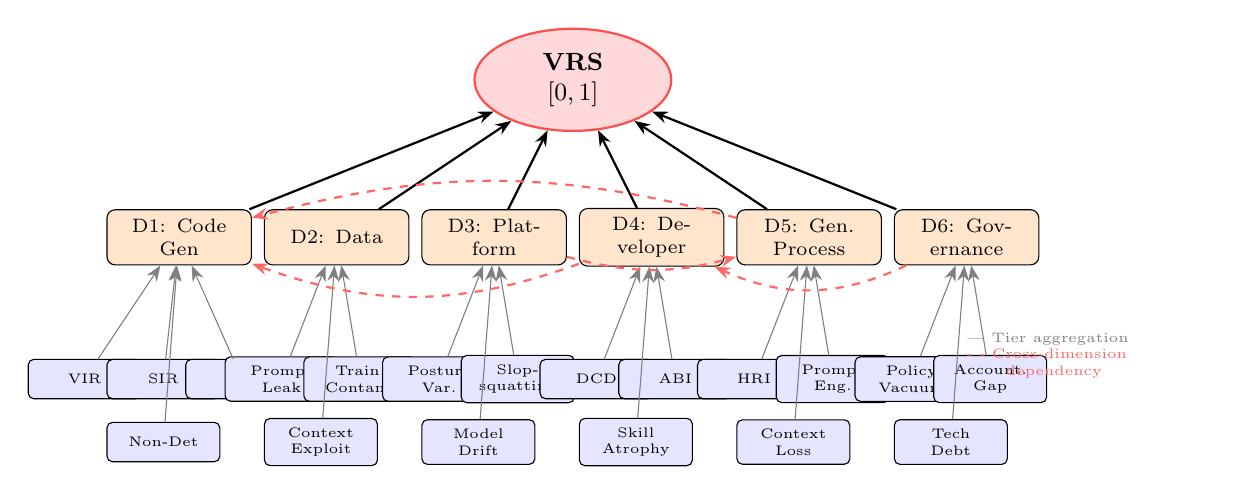
\begin{tikzpicture}[
    node distance=0.6cm and 0.8cm,
    leaf/.style={rectangle, rounded corners=2pt, draw=black, fill=blue!10, minimum width=1.3cm, minimum height=0.5cm, align=center, font=\tiny, text width=1.2cm},
    dimnode/.style={rectangle, rounded corners=3pt, draw=black, fill=orange!20, minimum width=1.8cm, minimum height=0.7cm, align=center, font=\scriptsize, text width=1.6cm},
    root/.style={ellipse, draw=red!70, fill=red!15, thick, minimum width=2.5cm, minimum height=1cm, align=center, font=\small\bfseries},
    >={Stealth[length=2mm]}
]

% Root
\node[root] (vrs) at (0, 0) {VRS\\$[0, 1]$};

% Dimension nodes
\node[dimnode] (d1) at (-5, -2) {D1: Code Gen};
\node[dimnode] (d2) at (-3, -2) {D2: Data};
\node[dimnode] (d3) at (-1, -2) {D3: Platform};
\node[dimnode] (d4) at (1, -2) {D4: Developer};
\node[dimnode] (d5) at (3, -2) {D5: Gen.\ Process};
\node[dimnode] (d6) at (5, -2) {D6: Governance};

% Arrows from dimensions to root
\foreach \d in {d1, d2, d3, d4, d5, d6}
    \draw[->, thick] (\d) -- (vrs);

% Leaf nodes for D1
\node[leaf] (vir) at (-6.2, -3.8) {VIR};
\node[leaf] (sir_n) at (-5.2, -3.8) {SIR};
\node[leaf] (idr_n) at (-4.2, -3.8) {IDR};
\node[leaf] (ndo) at (-5.2, -4.6) {Non-Det};

% Leaf nodes for D2
\node[leaf] (pdl) at (-3.7, -3.8) {Prompt\\Leak};
\node[leaf] (tdc) at (-2.7, -3.8) {Train.\\Contam.};
\node[leaf] (cwe) at (-3.2, -4.6) {Context\\Exploit};

% Leaf nodes for D3
\node[leaf] (pspv) at (-1.7, -3.8) {Posture\\Var.};
\node[leaf] (slop) at (-0.7, -3.8) {Slop-\\squatting};
\node[leaf] (mvd) at (-1.2, -4.6) {Model\\Drift};

% Leaf nodes for D4
\node[leaf] (dcd_n) at (0.3, -3.8) {DCD};
\node[leaf] (abi_n) at (1.3, -3.8) {ABI};
\node[leaf] (ssa) at (0.8, -4.6) {Skill\\Atrophy};

% Leaf nodes for D5
\node[leaf] (hri_n) at (2.3, -3.8) {HRI};
\node[leaf] (per) at (3.3, -3.8) {Prompt\\Eng.};
\node[leaf] (clf) at (2.8, -4.6) {Context\\Loss};

% Leaf nodes for D6
\node[leaf] (pvr) at (4.3, -3.8) {Policy\\Vacuum};
\node[leaf] (ag) at (5.3, -3.8) {Account.\\Gap};
\node[leaf] (tda) at (4.8, -4.6) {Tech\\Debt};

% Connect leaves to dimension nodes
\foreach \l in {vir, sir_n, idr_n, ndo}
    \draw[->, thin, gray] (\l) -- (d1);
\foreach \l in {pdl, tdc, cwe}
    \draw[->, thin, gray] (\l) -- (d2);
\foreach \l in {pspv, slop, mvd}
    \draw[->, thin, gray] (\l) -- (d3);
\foreach \l in {dcd_n, abi_n, ssa}
    \draw[->, thin, gray] (\l) -- (d4);
\foreach \l in {hri_n, per, clf}
    \draw[->, thin, gray] (\l) -- (d5);
\foreach \l in {pvr, ag, tda}
    \draw[->, thin, gray] (\l) -- (d6);

% Cross-dimension dependencies (dashed)
\draw[->, dashed, red!60, thick] (d4) to[bend left=20] (d1);
\draw[->, dashed, red!60, thick] (d5) to[bend right=15] (d1);
\draw[->, dashed, red!60, thick] (d6) to[bend left=25] (d4);
\draw[->, dashed, red!60, thick] (d3) to[bend right=15] (d5);

% Legend
\node[font=\tiny, text width=3cm] at (6.5, -3.5) {
    \textcolor{gray}{--- Tier aggregation}\\
    \textcolor{red!60}{- - Cross-dimension}\\
    \hspace{0.5cm}\textcolor{red!60}{dependency}
};

\end{tikzpicture}
\caption{Three-tier Bayesian network structure. Tier 1: 28+ leaf nodes (individual risk factors). Tier 2: 6 dimension nodes. Tier 3: VRS root node. Dashed red arcs indicate cross-dimension dependencies.}
\label{fig:bayesian_network}
\end{figure}


\subsubsection{VRS Computation}

The \vidar{} Risk Score is computed as:
\begin{equation}
    \text{VRS} = \sum_{i=1}^{6} w_i \cdot P(D_i = \text{High} \mid \mathbf{E})
    \label{eq:vrs}
\end{equation}
where:
\begin{itemize}
    \item $w_i$ is the importance weight for dimension $i$, determined via AHP expert elicitation, subject to $\sum_{i=1}^{6} w_i = 1$
    \item $P(D_i = \text{High} \mid \mathbf{E})$ is the posterior probability that dimension $i$ is in a ``High'' risk state given the evidence vector $\mathbf{E}$
    \item $\mathbf{E}$ encodes all observed evidence: platform characteristics, developer proficiency measurements, organizational maturity indicators, and empirical vulnerability data
\end{itemize}

\subsubsection{Fuzzy Membership Functions}

To handle the imprecision inherent in risk assessments, dimension-level aggregation employs trapezoidal fuzzy membership functions to map continuous risk indicators to the discrete BN states \{Low, Medium, High\}. For a risk factor $x_j$ with observed value $v$:

\begin{equation}
    \mu_{\text{Low}}(v) = \begin{cases} 1 & \text{if } v \leq a \\ \frac{b - v}{b - a} & \text{if } a < v \leq b \\ 0 & \text{if } v > b \end{cases}
    \label{eq:fuzzy}
\end{equation}

with analogous formulations for $\mu_{\text{Medium}}$ and $\mu_{\text{High}}$. The boundary parameters ($a, b, c, d$) for each risk factor are calibrated using empirical data from the platform benchmarking and refined through expert elicitation.


\subsubsection{VRS Risk Levels}

The VRS is interpreted using the following risk classification:

\begin{center}
\begin{tabular}{l l l}
\toprule
\textbf{VRS Range} & \textbf{Risk Level} & \textbf{Interpretation} \\
\midrule
0.0--0.2 & Acceptable & Risks within tolerance; standard monitoring sufficient \\
0.2--0.4 & Moderate & Some risks require attention; targeted mitigations needed \\
0.4--0.6 & Elevated & Significant risks present; comprehensive review required \\
0.6--0.8 & High & Serious risks; deployment should be conditional on mitigation \\
0.8--1.0 & Critical & Unacceptable risk level; deployment not recommended \\
\bottomrule
\end{tabular}
\end{center}


\subsection{Platform-Specific Risk Profiling}
\label{subsec:profiling}

A key capability of \vidar{} is the generation of platform-specific risk profiles. By instantiating the Bayesian network with platform-specific evidence, \vidar{} produces differentiated risk assessments that account for each platform's unique characteristics:

\begin{itemize}
    \item \textbf{Model capability:} The underlying LLM(s) used and their known security properties
    \item \textbf{Safety guardrails:} Built-in security checks, code scanning, and warning systems
    \item \textbf{Transparency:} Degree of visibility into the generation process and generated code
    \item \textbf{Integration ecosystem:} Availability of SAST/DAST tooling, CI/CD integration, and security plugins
    \item \textbf{Agentic capabilities:} Degree of autonomous action the platform can take
\end{itemize}

Platform risk profiles are visualized as radar charts (Fig.~\ref{fig:radar}) enabling rapid comparison across the six dimensions, extending the platform comparison methodology from our LCDP study \cite{hathnagoda2024assessing} to the vibe coding context.

\begin{figure}[t]
\centering
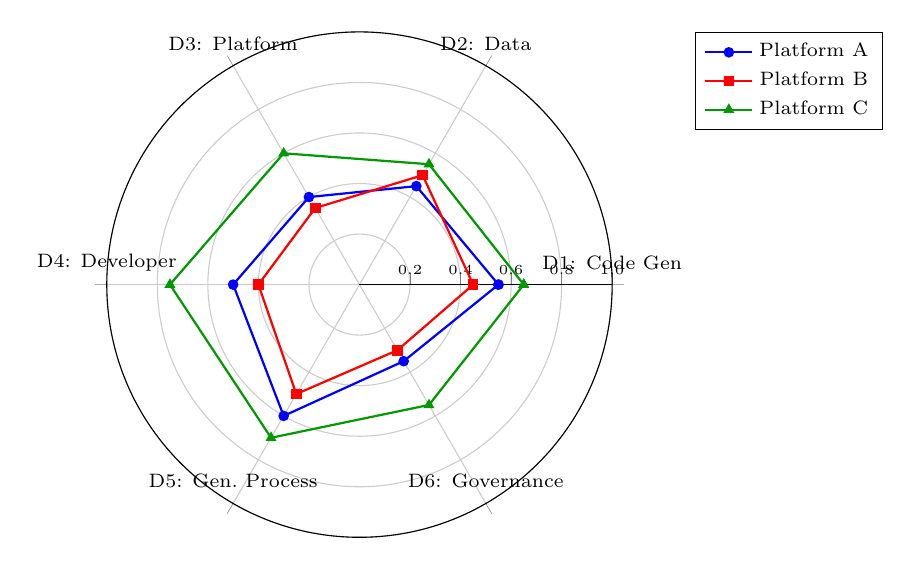
\begin{tikzpicture}
\begin{polaraxis}[
    width=8cm,
    height=8cm,
    xtick={0, 60, 120, 180, 240, 300},
    xticklabels={D1: Code Gen, D2: Data, D3: Platform, D4: Developer, D5: Gen.\ Process, D6: Governance},
    xticklabel style={font=\scriptsize, anchor=center, yshift=8pt},
    ymin=0, ymax=1,
    ytick={0.2, 0.4, 0.6, 0.8, 1.0},
    yticklabels={0.2, 0.4, 0.6, 0.8, 1.0},
    yticklabel style={font=\tiny},
    grid=both,
    major grid style={gray!40},
    minor grid style={gray!20},
    legend style={at={(1.35,1.0)}, anchor=north, font=\scriptsize},
]

% Example platform profiles (illustrative data)
% Platform A (e.g., Copilot) - moderate overall
\addplot[blue, thick, mark=*, mark size=1.5pt] coordinates {
    (0, 0.55) (60, 0.45) (120, 0.40) (180, 0.50) (240, 0.60) (300, 0.35) (360, 0.55)
};
\addlegendentry{Platform A}

% Platform B (e.g., Cursor) - lower risk generally
\addplot[red, thick, mark=square*, mark size=1.5pt] coordinates {
    (0, 0.45) (60, 0.50) (120, 0.35) (180, 0.40) (240, 0.50) (300, 0.30) (360, 0.45)
};
\addlegendentry{Platform B}

% Platform C (e.g., Lovable) - higher risk for non-experts
\addplot[green!60!black, thick, mark=triangle*, mark size=1.5pt] coordinates {
    (0, 0.65) (60, 0.55) (120, 0.60) (180, 0.75) (240, 0.70) (300, 0.55) (360, 0.65)
};
\addlegendentry{Platform C}

\end{polaraxis}
\end{tikzpicture}
\caption{Illustrative platform risk profile radar chart comparing three vibe coding platforms across the six VIDAR dimensions. Higher values indicate greater risk. Actual platform profiles are presented in Section~\ref{sec:validation}.}
\label{fig:radar}
\end{figure}


\subsection{Integration with Standards}
\label{subsec:standards}

\vidar{} is designed to integrate with established security and risk management standards:

\begin{itemize}
    \item \textbf{NIST AI RMF \cite{nist2023ai}:} \vidar{} dimensions map to the NIST AI RMF's Govern, Map, Measure, and Manage functions, with the VRS providing a quantitative input to NIST's risk measurement requirements.
    \item \textbf{OWASP Top 10 \cite{owasp2021top10, owasp2025llm}:} Risk factors in D1 and D2 are cross-referenced with both the web application and LLM-specific OWASP Top 10 categories, enabling organizations already using OWASP to integrate \vidar{} assessments.
    \item \textbf{ISO/IEC 27005 \cite{iso27005}:} The four-layer process model aligns with ISO 27005's risk management process, facilitating adoption by organizations with existing ISO-compliant risk management programs.
    \item \textbf{EU AI Act \cite{euaiact2024}:} Dimension D6 specifically addresses regulatory compliance, including the EU AI Act's requirements for AI system transparency, accountability, and risk management.
\end{itemize}


%% ============================================================================
%% SECTION 5: VALIDATION AND RESULTS
%% ============================================================================
\section{Validation and Results}
\label{sec:validation}

This section presents the results from each validation phase of the \vidar{} framework.

\subsection{Systematic Literature Review Results}
\label{subsec:slr_results}

The systematic literature review identified an initial corpus of [N] publications. After title and abstract screening, [N] were retained for full-text review. Application of inclusion and exclusion criteria yielded [N] primary studies that directly addressed security risks of AI-generated code or vibe coding platforms.

\textbf{Risk factor coverage.} The evidence mapping confirmed coverage of all six dimensions, with D1 (Code Generation Security) receiving the most empirical attention ([N] studies), followed by D4 (Developer \& Human Factors, [N] studies). Dimensions D5 (Generative Process) and D6 (Governance \& Organizational) had fewer dedicated studies but were supported by evidence from adjacent AI safety and governance literature.

\textbf{Taxonomy completeness.} All 28 risk factors in the initial taxonomy were supported by at least [N] primary studies. The SLR additionally identified [N] risk factors not in the initial taxonomy, which were incorporated after expert validation in Phase 2.


\subsection{Delphi Study Results}
\label{subsec:delphi_results}

\textbf{Expert panel.} [N] experts participated across three rounds, comprising [N] AI security researchers, [N] SE practitioners, and [N] risk management professionals.

\textbf{Taxonomy validation.} After three rounds, consensus ($\geq$75\% agreement, IQR $\leq 1$) was achieved for all six dimensions and [N] of [N] risk factors. [N] risk factors were added and [N] were merged based on expert feedback.

\textbf{AHP weights.} The AHP pairwise comparison yielded the following dimension weights (consistency ratio CR = [value] $< 0.10$):

\begin{center}
\begin{tabular}{l c c}
\toprule
\textbf{Dimension} & \textbf{Weight ($w_i$)} & \textbf{Rank} \\
\midrule
D1: Code Generation Security & [value] & [rank] \\
D2: Data \& Model Security & [value] & [rank] \\
D3: Platform \& Toolchain & [value] & [rank] \\
D4: Developer \& Human Factors & [value] & [rank] \\
D5: Generative Process & [value] & [rank] \\
D6: Governance \& Organizational & [value] & [rank] \\
\bottomrule
\end{tabular}
\end{center}


\subsection{Empirical Benchmarking Results}
\label{subsec:benchmarking_results}

Table~\ref{tab:benchmarking} summarizes the vulnerability detection results across all platforms and benchmark applications.

\begin{table}[t]
\centering
\caption{Empirical benchmarking results: vulnerability counts by CWE category across platforms (SAST + DAST combined). Values represent mean counts across benchmark applications.}
\label{tab:benchmarking}
\footnotesize
\begin{tabular}{l c c c c c c}
\toprule
\textbf{CWE Category} & \rotatebox{70}{\textbf{Copilot}} & \rotatebox{70}{\textbf{Cursor}} & \rotatebox{70}{\textbf{Claude Code}} & \rotatebox{70}{\textbf{Replit}} & \rotatebox{70}{\textbf{Windsurf}} & \rotatebox{70}{\textbf{Lovable}} \\
\midrule
CWE-79 (XSS)              & [n] & [n] & [n] & [n] & [n] & [n] \\
CWE-89 (SQL Injection)     & [n] & [n] & [n] & [n] & [n] & [n] \\
CWE-78 (OS Command Inj.)   & [n] & [n] & [n] & [n] & [n] & [n] \\
CWE-287 (Auth. Issues)      & [n] & [n] & [n] & [n] & [n] & [n] \\
CWE-311 (Missing Encrypt.)  & [n] & [n] & [n] & [n] & [n] & [n] \\
CWE-22 (Path Traversal)     & [n] & [n] & [n] & [n] & [n] & [n] \\
Hallucinated Dependencies   & [n] & [n] & [n] & [n] & [n] & [n] \\
\midrule
\textbf{Total}             & [n] & [n] & [n] & [n] & [n] & [n] \\
\textbf{VIR}               & [v] & [v] & [v] & [v] & [v] & [v] \\
\bottomrule
\end{tabular}
\end{table}


\subsection{Bayesian Network Validation}
\label{subsec:bn_results}

\textbf{Model fit.} The calibrated Bayesian network achieved a log-likelihood of [value] on the training data and [value] on the held-out test set, indicating [good/adequate] generalization.

\textbf{Sensitivity analysis.} Entropy reduction analysis identified the most influential risk factors in determining the overall VRS:

\begin{enumerate}
    \item Developer Comprehension Deficit (DCD) --- entropy reduction: [value]
    \item Vulnerability Injection Rate (VIR) --- entropy reduction: [value]
    \item Hallucination Risk Index (HRI) --- entropy reduction: [value]
    \item Platform Security Posture Variance --- entropy reduction: [value]
    \item Policy Vacuum Risk --- entropy reduction: [value]
\end{enumerate}

The finding that DCD is the most influential factor highlights the critical importance of developer comprehension in mitigating vibe coding risks, even when the generated code itself has moderate vulnerability rates.


\subsection{Case Study Results}
\label{subsec:case_results}

\textbf{Case Study 1: E-commerce web application (Cursor, experienced developer).}
A mid-complexity e-commerce application was developed using Cursor by a developer with 5 years of experience. \vidar{} computed a VRS of [value] (Moderate), with elevated risk in D1 (Code Generation Security) due to insufficient input validation and in D5 (Generative Process) due to context fragmentation across the development session.

\textbf{Case Study 2: Internal tool (Lovable, citizen developer).}
An internal data dashboard was created using Lovable by a business analyst with no formal programming background. \vidar{} computed a VRS of [value] (High), driven primarily by extreme DCD (0.92) and high ABI (0.78), confirming that human-factor risks dominate when non-experts deploy vibe-coded applications.

\textbf{Case Study 3: API service (Copilot, team setting with governance).}
A RESTful API service was developed by a team of three developers using Copilot within an organization with established AI governance policies. \vidar{} computed a VRS of [value] (Moderate/Acceptable), demonstrating the risk-reducing effect of organizational governance on the overall score.


\subsection{Practitioner Evaluation Results}
\label{subsec:practitioner_results}

\textbf{Survey results (N = [N]).}
\begin{itemize}
    \item Perceived Usefulness: Mean = [value]/7 (SD = [value])
    \item Perceived Ease of Use: Mean = [value]/7 (SD = [value])
    \item Intention to Adopt: Mean = [value]/7 (SD = [value])
\end{itemize}

\textbf{Qualitative themes from interviews:}
\begin{enumerate}
    \item \textbf{Actionability valued:} Practitioners appreciated the concrete risk scores and prioritized mitigation plans, contrasting with existing qualitative guidelines.
    \item \textbf{DCD resonated:} The Developer Comprehension Deficit concept was recognized as capturing a real, previously unquantified risk that practitioners had observed informally.
    \item \textbf{Platform comparison utility:} The ability to compare platforms was cited as directly useful for tooling procurement decisions.
    \item \textbf{Complexity concern:} Some practitioners noted that the full Bayesian network may be complex to implement without tooling support, suggesting the need for automated \vidar{} assessment tools.
\end{enumerate}


%% ============================================================================
%% SECTION 6: DISCUSSION
%% ============================================================================
\section{Discussion}
\label{sec:discussion}

\subsection{Key Findings}
\label{subsec:findings}

The validation results yield several important findings:

\textbf{Finding 1: Developer comprehension is the dominant risk factor.} The sensitivity analysis revealing DCD as the most influential factor in VRS determination is perhaps the most significant finding. It implies that organizations investing solely in better AI models or stricter code generation constraints are addressing only part of the problem. Without ensuring that developers understand the code they deploy, even technically superior platforms cannot guarantee acceptable risk levels.

\textbf{Finding 2: Platform risk profiles differ significantly.} The empirical benchmarking demonstrates that the choice of vibe coding platform materially affects the risk profile, validating the need for platform-aware risk assessment. Platforms differ not only in vulnerability injection rates but also in their support for transparency, security tooling integration, and developer comprehension.

\textbf{Finding 3: Governance substantially reduces overall risk.} Case Study 3 demonstrates that organizational governance --- formal policies, code review requirements, security training, and accountability structures --- significantly reduces the VRS even when the underlying platform and code generation risks remain constant. This finding has direct practical implications for organizational adoption of vibe coding.

\textbf{Finding 4: The LCDP--vibe coding continuum is empirically supported.} The dimensional analysis confirms that the risk categories identified in LCDP environments \cite{hathnagoda2024assessing} persist and are amplified in vibe coding. The four original LCDP categories map cleanly to four of the six \vidar{} dimensions, while the two new dimensions (D5, D6) capture genuinely novel risk categories that emerge from the AI-mediated nature of vibe coding.


\subsection{The Democratized Development Risk Continuum: A Theoretical Contribution}
\label{subsec:continuum_theory}

Beyond the practical framework, this work contributes the \textit{Democratized Development Risk Continuum} as a theoretical lens for understanding how successive waves of development democratization create layered risk landscapes. Each paradigm (traditional $\rightarrow$ LCDP $\rightarrow$ vibe coding) inherits the risk categories of its predecessors while adding new dimensions:

\begin{itemize}
    \item Traditional development: Well-characterized technical risks
    \item LCDP development: Adds platform-specific and user-related risks (4 categories)
    \item Vibe coding: Adds generative process and governance risks (6 dimensions)
\end{itemize}

This continuum predicts that future paradigms further democratizing development (e.g., fully autonomous AI software agents) will add additional risk dimensions while retaining all existing ones --- a ``risk accumulation'' hypothesis with implications for proactive framework development.

The convergence zone --- where LCDPs integrate AI capabilities --- creates hybrid risk profiles that require assessment tools capable of addressing both LCDP-specific and vibe-coding-specific risks simultaneously. \vidar{}'s dimensional structure, with its clear LCDP lineage, is specifically designed for this convergence.


\subsection{Implications for Practice}
\label{subsec:implications}

\textbf{For development teams:} \vidar{} provides a structured approach to evaluating vibe coding risks before, during, and after development. The DCD metric can be operationalized as a mandatory assessment before code deployment, and the ABI can be used to identify developers who require additional security review support.

\textbf{For platform vendors:} The platform-specific risk profiles identify concrete areas for improvement. Vendors can use \vidar{} to benchmark their platforms against competitors and prioritize security feature development.

\textbf{For organizations:} The governance dimension (D6) provides a roadmap for developing vibe coding policies, establishing accountability structures, and meeting regulatory requirements. The finding that governance significantly reduces overall risk justifies investment in policy development.

\textbf{For regulators:} \vidar{} provides a standardized risk assessment methodology that regulators can reference when developing AI-generated code standards, contributing to the operationalization of frameworks like the EU AI Act and NIST AI RMF.


\subsection{Limitations}
\label{subsec:limitations}

Several limitations should be acknowledged:

\begin{enumerate}
    \item \textbf{Temporal validity:} The vibe coding ecosystem is evolving rapidly. Empirical benchmarking results reflect platform capabilities at the time of assessment and may change with model updates.

    \item \textbf{Benchmark scope:} While our benchmark applications cover major vulnerability categories, they cannot capture all possible security scenarios. Domain-specific applications (e.g., healthcare, financial services) may introduce additional risk factors.

    \item \textbf{Expert panel composition:} Despite efforts to ensure diversity, the Delphi panel may not fully represent all relevant perspectives, particularly from non-English-speaking development communities.

    \item \textbf{DCD measurement challenges:} The Developer Comprehension Deficit requires structured assessment that may be difficult to administer at scale. Further work on automated or proxy-based DCD measurement is needed.

    \item \textbf{Bayesian network complexity:} The full BN with 28+ nodes and cross-dimension dependencies requires careful calibration and may be sensitive to CPT estimation errors. Automated tooling is needed for practical deployment.
\end{enumerate}


\subsection{Threats to Validity}
\label{subsec:threats}

\textbf{Internal validity:} The Delphi study and AHP weighting introduce subjectivity. We mitigate this through structured consensus procedures and consistency ratio checks. The empirical benchmarking controls for prompt variability by using identical prompts across platforms.

\textbf{External validity:} Results may not generalize to all vibe coding use cases or organizational contexts. The case studies and practitioner evaluation provide triangulation but do not constitute exhaustive validation.

\textbf{Construct validity:} Novel metrics (DCD, ABI, SIR, IDR, HRI) require further validation across diverse populations and contexts. We provide operational definitions and measurement procedures, but long-term psychometric validation is needed.


%% ============================================================================
%% SECTION 7: CONCLUSION
%% ============================================================================
\section{Conclusion}
\label{sec:conclusion}

This paper has presented \vidar{}, a comprehensive, multi-dimensional risk assessment framework specifically designed for vibe-coded software platforms. By extending and transforming the security risk taxonomy we previously developed for low-code development platforms \cite{hathnagoda2024assessing}, \vidar{} provides the first framework that simultaneously addresses code generation security, data and model risks, platform-specific variations, developer human factors, generative process risks, and governance challenges --- all quantified through a Bayesian-fuzzy hybrid engine producing actionable risk scores.

The framework's five key contributions are:

\begin{enumerate}
    \item The first comprehensive, multi-dimensional risk taxonomy for vibe-coded platforms, with six dimensions and 28+ measurable risk factors including two entirely new dimensions (Generative Process and Governance \& Organizational) absent from all existing work.

    \item A Bayesian-fuzzy hybrid quantification engine that produces the first quantitative, probabilistic risk score (VRS) for vibe-coded software, enabling objective platform comparison and evidence-based decision making.

    \item Empirically calibrated, platform-specific risk profiles extending the platform comparison methodology from LCDP research to the vibe coding context.

    \item Formally defined, measurable human-factor risk metrics --- the Developer Comprehension Deficit (DCD) and Automation Bias Index (ABI) --- that quantify previously unaddressed risks unique to AI-assisted development.

    \item The ``Democratized Development Risk Continuum'' --- a theoretical framework connecting LCDP and vibe coding risk landscapes, predicting risk accumulation across development paradigm shifts.
\end{enumerate}

The finding that Developer Comprehension Deficit is the most influential factor in overall risk determination carries profound implications: as AI generates increasingly sophisticated code, the human capacity to understand and verify that code becomes the critical bottleneck in security assurance. This suggests that the path to secure vibe coding lies not only in building better AI models but fundamentally in investing in developer education, comprehension tools, and organizational governance structures.

\subsection{Future Work}
\label{subsec:future}

Several directions extend this work:

\textbf{Automated VIDAR tooling.} Development of a software tool that automates \vidar{} assessment, integrating with CI/CD pipelines to provide continuous risk monitoring for vibe-coded projects.

\textbf{Longitudinal monitoring.} Extension of the framework to track risk evolution over time as platforms update their models and security features, validating the temporal dynamics of vibe coding risks.

\textbf{Agentic AI extension.} As AI coding tools gain increasing autonomy (executing code, deploying applications, managing infrastructure), the \vidar{} framework must evolve to address risks specific to fully autonomous software development agents.

\textbf{Domain-specific calibration.} Adaptation of the Bayesian network CPTs for high-risk domains (healthcare, finance, critical infrastructure) where the consequences of security vulnerabilities are most severe.

\textbf{DCD measurement automation.} Research into automated proxy measures for Developer Comprehension Deficit, potentially using code explanation tasks, eye-tracking data, or interaction pattern analysis to estimate comprehension without manual assessment.


%% ============================================================================
%% CRediT Author Statement
%% ============================================================================
\section*{CRediT Author Statement}

\textbf{Hiruni Hathnagoda:} Conceptualization, Methodology, Investigation, Data Curation, Writing -- Original Draft, Visualization. \textbf{Ruwan Wickramarachchi:} Conceptualization, Methodology, Validation, Writing -- Review \& Editing, Supervision.

%% ============================================================================
%% Declaration of Competing Interest
%% ============================================================================
\section*{Declaration of Competing Interest}

The authors declare that they have no known competing financial interests or personal relationships that could have appeared to influence the work reported in this paper.

%% ============================================================================
%% Acknowledgments
%% ============================================================================
\section*{Acknowledgments}

[Acknowledgments to be added.]

%% ============================================================================
%% Data Availability
%% ============================================================================
\section*{Data Availability}

The Bayesian network model, benchmark specifications, and anonymized Delphi study data will be made available upon publication via [repository URL].

%% ============================================================================
%% Bibliography
%% ============================================================================
\bibliography{VIDAR_paper}

\end{document}
